\chapter{Appendix A}
\label{text:appendixa}

Full Cancer Informatics SQL for PostgreSQL

The following SQL scripts for PostgreSQL will deploy the empty Cancer.Informatics schema that is required to store the source system data for the data crawlers to process into the Smart Health Data Vault (SHDV)

\begin{lstlisting}

-- Database generated with pgModeler (PostgreSQL Database Modeler).
-- pgModeler  version: 0.9.2-alpha1
-- PostgreSQL version: 11.0
-- Project Site: pgmodeler.io
-- Model Author: ---


-- Database creation must be done outside a multicommand file.
-- These commands were put in this file only as a convenience.
-- -- object: dv_chemocare_treatment_db | type: DATABASE --
-- -- DROP DATABASE IF EXISTS dv_chemocare_treatment_db;
-- CREATE DATABASE dv_chemocare_treatment_db;
-- -- ddl-end --
-- 

-- object: public.hub_person | type: TABLE --
-- DROP TABLE IF EXISTS public.hub_person CASCADE;
CREATE TABLE public.hub_person (
	chi int4 NOT NULL GENERATED ALWAYS AS IDENTITY ,
	CONSTRAINT hub_person_pk PRIMARY KEY (chi)

);
-- ddl-end --
ALTER TABLE public.hub_person OWNER TO postgres;
-- ddl-end --

-- object: public.hub_time | type: TABLE --
-- DROP TABLE IF EXISTS public.hub_time CASCADE;
CREATE TABLE public.hub_time (
	id serial NOT NULL,
	CONSTRAINT hub_time_pk PRIMARY KEY (id)

);
-- ddl-end --
ALTER TABLE public.hub_time OWNER TO postgres;
-- ddl-end --

-- object: public.sat_person_patient_measurements | type: TABLE --
-- DROP TABLE IF EXISTS public.sat_person_patient_measurements CASCADE;
CREATE TABLE public.sat_person_patient_measurements (
	id serial NOT NULL,
	age_at_diagnosis float,
	height decimal(3,2),
	weight decimal(4,1),
	surface_area decimal(3,2),
	chi_hub_person int4 NOT NULL,
	CONSTRAINT sat_person_patient_measurements_pk PRIMARY KEY (id)

);
-- ddl-end --
ALTER TABLE public.sat_person_patient_measurements OWNER TO postgres;
-- ddl-end --

-- object: public.hub_object | type: TABLE --
-- DROP TABLE IF EXISTS public.hub_object CASCADE;
CREATE TABLE public.hub_object (
	id serial NOT NULL,
	CONSTRAINT hub_object_pk PRIMARY KEY (id)

);
-- ddl-end --
ALTER TABLE public.hub_object OWNER TO postgres;
-- ddl-end --

-- object: public.sat_time_appointment_date | type: TABLE --
-- DROP TABLE IF EXISTS public.sat_time_appointment_date CASCADE;
CREATE TABLE public.sat_time_appointment_date (
	id serial NOT NULL,
	appointment_date date,
	id_hub_time integer NOT NULL,
	CONSTRAINT sat_time_appointment_date_pk PRIMARY KEY (id)

);
-- ddl-end --
ALTER TABLE public.sat_time_appointment_date OWNER TO postgres;
-- ddl-end --

-- object: public."sat_time_last-toxicity_date" | type: TABLE --
-- DROP TABLE IF EXISTS public."sat_time_last-toxicity_date" CASCADE;
CREATE TABLE public."sat_time_last-toxicity_date" (
	id serial NOT NULL,
	last_toxicity_date date,
	id_hub_time integer NOT NULL,
	CONSTRAINT "sat_time_last-toxicity_date_pk" PRIMARY KEY (id)

);
-- ddl-end --
ALTER TABLE public."sat_time_last-toxicity_date" OWNER TO postgres;
-- ddl-end --

-- object: public.sat_object_tumour_group | type: TABLE --
-- DROP TABLE IF EXISTS public.sat_object_tumour_group CASCADE;
CREATE TABLE public.sat_object_tumour_group (
	id serial NOT NULL,
	tumour_group varchar(255),
	id_hub_object integer NOT NULL,
	CONSTRAINT sat_object_tumour_group_pk PRIMARY KEY (id)

);
-- ddl-end --
ALTER TABLE public.sat_object_tumour_group OWNER TO postgres;
-- ddl-end --

-- object: public.sat_person_consultant_chemo | type: TABLE --
-- DROP TABLE IF EXISTS public.sat_person_consultant_chemo CASCADE;
CREATE TABLE public.sat_person_consultant_chemo (
	id serial NOT NULL,
	consultant_code char(2),
	chi_hub_person int4 NOT NULL,
	CONSTRAINT sat_person_consultant_chemo_pk PRIMARY KEY (id)

);
-- ddl-end --
ALTER TABLE public.sat_person_consultant_chemo OWNER TO postgres;
-- ddl-end --

-- object: public.hub_event | type: TABLE --
-- DROP TABLE IF EXISTS public.hub_event CASCADE;
CREATE TABLE public.hub_event (
	id serial NOT NULL,
	CONSTRAINT hub_event_pk PRIMARY KEY (id)

);
-- ddl-end --
ALTER TABLE public.hub_event OWNER TO postgres;
-- ddl-end --

-- object: public.sat_object_drug_details | type: TABLE --
-- DROP TABLE IF EXISTS public.sat_object_drug_details CASCADE;
CREATE TABLE public.sat_object_drug_details (
	id serial NOT NULL,
	drug_type char(9),
	drug_name varchar(255),
	given_drug decimal(72),
	drug_dose decimal(7,2),
	required_dose decimal(7,2),
	id_hub_object integer NOT NULL,
	CONSTRAINT sat_object_drug_details_pk PRIMARY KEY (id)

);
-- ddl-end --
ALTER TABLE public.sat_object_drug_details OWNER TO postgres;
-- ddl-end --

-- object: public.sat_object_treatment_details | type: TABLE --
-- DROP TABLE IF EXISTS public.sat_object_treatment_details CASCADE;
CREATE TABLE public.sat_object_treatment_details (
	id serial NOT NULL,
	intention varchar(255),
	regime varchar(255),
	cycle int4,
	id_hub_object integer NOT NULL,
	CONSTRAINT sat_object_treatment_details_pk PRIMARY KEY (id)

);
-- ddl-end --
ALTER TABLE public.sat_object_treatment_details OWNER TO postgres;
-- ddl-end --

-- object: public.sat_event_drug_status | type: TABLE --
-- DROP TABLE IF EXISTS public.sat_event_drug_status CASCADE;
CREATE TABLE public.sat_event_drug_status (
	id serial NOT NULL,
	drug_status varchar(255),
	id_hub_event integer NOT NULL,
	CONSTRAINT sat_event_drug_status_pk PRIMARY KEY (id)

);
-- ddl-end --
ALTER TABLE public.sat_event_drug_status OWNER TO postgres;
-- ddl-end --

-- object: public.many_hub_person_has_many_hub_time | type: TABLE --
-- DROP TABLE IF EXISTS public.many_hub_person_has_many_hub_time CASCADE;
CREATE TABLE public.many_hub_person_has_many_hub_time (
	chi_hub_person int4 NOT NULL,
	id_hub_time integer NOT NULL,
	id serial NOT NULL,
	CONSTRAINT many_hub_person_has_many_hub_time_pk PRIMARY KEY (id)

);
-- ddl-end --

-- object: hub_person_fk | type: CONSTRAINT --
-- ALTER TABLE public.many_hub_person_has_many_hub_time DROP CONSTRAINT IF EXISTS hub_person_fk CASCADE;
ALTER TABLE public.many_hub_person_has_many_hub_time ADD CONSTRAINT hub_person_fk FOREIGN KEY (chi_hub_person)
REFERENCES public.hub_person (chi) MATCH FULL
ON DELETE RESTRICT ON UPDATE CASCADE;
-- ddl-end --

-- object: hub_time_fk | type: CONSTRAINT --
-- ALTER TABLE public.many_hub_person_has_many_hub_time DROP CONSTRAINT IF EXISTS hub_time_fk CASCADE;
ALTER TABLE public.many_hub_person_has_many_hub_time ADD CONSTRAINT hub_time_fk FOREIGN KEY (id_hub_time)
REFERENCES public.hub_time (id) MATCH FULL
ON DELETE RESTRICT ON UPDATE CASCADE;
-- ddl-end --

-- object: public.many_hub_person_has_many_hub_object | type: TABLE --
-- DROP TABLE IF EXISTS public.many_hub_person_has_many_hub_object CASCADE;
CREATE TABLE public.many_hub_person_has_many_hub_object (
	chi_hub_person int4 NOT NULL,
	id_hub_object integer NOT NULL,
	id serial NOT NULL,
	CONSTRAINT many_hub_person_has_many_hub_object_pk PRIMARY KEY (id)

);
-- ddl-end --

-- object: hub_person_fk | type: CONSTRAINT --
-- ALTER TABLE public.many_hub_person_has_many_hub_object DROP CONSTRAINT IF EXISTS hub_person_fk CASCADE;
ALTER TABLE public.many_hub_person_has_many_hub_object ADD CONSTRAINT hub_person_fk FOREIGN KEY (chi_hub_person)
REFERENCES public.hub_person (chi) MATCH FULL
ON DELETE RESTRICT ON UPDATE CASCADE;
-- ddl-end --

-- object: hub_object_fk | type: CONSTRAINT --
-- ALTER TABLE public.many_hub_person_has_many_hub_object DROP CONSTRAINT IF EXISTS hub_object_fk CASCADE;
ALTER TABLE public.many_hub_person_has_many_hub_object ADD CONSTRAINT hub_object_fk FOREIGN KEY (id_hub_object)
REFERENCES public.hub_object (id) MATCH FULL
ON DELETE RESTRICT ON UPDATE CASCADE;
-- ddl-end --

-- object: public.many_hub_person_has_many_hub_event | type: TABLE --
-- DROP TABLE IF EXISTS public.many_hub_person_has_many_hub_event CASCADE;
CREATE TABLE public.many_hub_person_has_many_hub_event (
	chi_hub_person int4 NOT NULL,
	id_hub_event integer NOT NULL,
	id serial NOT NULL,
	CONSTRAINT many_hub_person_has_many_hub_event_pk PRIMARY KEY (id)

);
-- ddl-end --

-- object: hub_person_fk | type: CONSTRAINT --
-- ALTER TABLE public.many_hub_person_has_many_hub_event DROP CONSTRAINT IF EXISTS hub_person_fk CASCADE;
ALTER TABLE public.many_hub_person_has_many_hub_event ADD CONSTRAINT hub_person_fk FOREIGN KEY (chi_hub_person)
REFERENCES public.hub_person (chi) MATCH FULL
ON DELETE RESTRICT ON UPDATE CASCADE;
-- ddl-end --

-- object: hub_event_fk | type: CONSTRAINT --
-- ALTER TABLE public.many_hub_person_has_many_hub_event DROP CONSTRAINT IF EXISTS hub_event_fk CASCADE;
ALTER TABLE public.many_hub_person_has_many_hub_event ADD CONSTRAINT hub_event_fk FOREIGN KEY (id_hub_event)
REFERENCES public.hub_event (id) MATCH FULL
ON DELETE RESTRICT ON UPDATE CASCADE;
-- ddl-end --

-- object: hub_person_fk | type: CONSTRAINT --
-- ALTER TABLE public.sat_person_consultant_chemo DROP CONSTRAINT IF EXISTS hub_person_fk CASCADE;
ALTER TABLE public.sat_person_consultant_chemo ADD CONSTRAINT hub_person_fk FOREIGN KEY (chi_hub_person)
REFERENCES public.hub_person (chi) MATCH FULL
ON DELETE RESTRICT ON UPDATE CASCADE;
-- ddl-end --

-- object: hub_person_fk | type: CONSTRAINT --
-- ALTER TABLE public.sat_person_patient_measurements DROP CONSTRAINT IF EXISTS hub_person_fk CASCADE;
ALTER TABLE public.sat_person_patient_measurements ADD CONSTRAINT hub_person_fk FOREIGN KEY (chi_hub_person)
REFERENCES public.hub_person (chi) MATCH FULL
ON DELETE RESTRICT ON UPDATE CASCADE;
-- ddl-end --

-- object: hub_time_fk | type: CONSTRAINT --
-- ALTER TABLE public."sat_time_last-toxicity_date" DROP CONSTRAINT IF EXISTS hub_time_fk CASCADE;
ALTER TABLE public."sat_time_last-toxicity_date" ADD CONSTRAINT hub_time_fk FOREIGN KEY (id_hub_time)
REFERENCES public.hub_time (id) MATCH FULL
ON DELETE RESTRICT ON UPDATE CASCADE;
-- ddl-end --

-- object: hub_time_fk | type: CONSTRAINT --
-- ALTER TABLE public.sat_time_appointment_date DROP CONSTRAINT IF EXISTS hub_time_fk CASCADE;
ALTER TABLE public.sat_time_appointment_date ADD CONSTRAINT hub_time_fk FOREIGN KEY (id_hub_time)
REFERENCES public.hub_time (id) MATCH FULL
ON DELETE RESTRICT ON UPDATE CASCADE;
-- ddl-end --

-- object: hub_object_fk | type: CONSTRAINT --
-- ALTER TABLE public.sat_object_tumour_group DROP CONSTRAINT IF EXISTS hub_object_fk CASCADE;
ALTER TABLE public.sat_object_tumour_group ADD CONSTRAINT hub_object_fk FOREIGN KEY (id_hub_object)
REFERENCES public.hub_object (id) MATCH FULL
ON DELETE RESTRICT ON UPDATE CASCADE;
-- ddl-end --

-- object: hub_object_fk | type: CONSTRAINT --
-- ALTER TABLE public.sat_object_drug_details DROP CONSTRAINT IF EXISTS hub_object_fk CASCADE;
ALTER TABLE public.sat_object_drug_details ADD CONSTRAINT hub_object_fk FOREIGN KEY (id_hub_object)
REFERENCES public.hub_object (id) MATCH FULL
ON DELETE RESTRICT ON UPDATE CASCADE;
-- ddl-end --

-- object: hub_object_fk | type: CONSTRAINT --
-- ALTER TABLE public.sat_object_treatment_details DROP CONSTRAINT IF EXISTS hub_object_fk CASCADE;
ALTER TABLE public.sat_object_treatment_details ADD CONSTRAINT hub_object_fk FOREIGN KEY (id_hub_object)
REFERENCES public.hub_object (id) MATCH FULL
ON DELETE RESTRICT ON UPDATE CASCADE;
-- ddl-end --

-- object: hub_event_fk | type: CONSTRAINT --
-- ALTER TABLE public.sat_event_drug_status DROP CONSTRAINT IF EXISTS hub_event_fk CASCADE;
ALTER TABLE public.sat_event_drug_status ADD CONSTRAINT hub_event_fk FOREIGN KEY (id_hub_event)
REFERENCES public.hub_event (id) MATCH FULL
ON DELETE RESTRICT ON UPDATE CASCADE;
-- ddl-end --

\end{lstlisting}


\chapter{Appendix B}
\label{text:appendixb}

Full Cancer Informatics SQL for MySQL

The following SQL scripts for MySQL will deploy the empty Cancer.Informatics schema that is required to store the source system data for the data crawlers to process into the Smart Health Data Vault (SHDV)

\begin{lstlisting}
CREATE TABLE `hub_event` (
  `id` integer,
  PRIMARY KEY (`id`)
);

CREATE TABLE `hub_object` (
  `id` integer,
  PRIMARY KEY (`id`)
);

CREATE TABLE `hub_person` (
  `chi` integer,
  PRIMARY KEY (`chi`)
);

CREATE TABLE `hub_time` (
  `id` integer,
  PRIMARY KEY (`id`)
);

CREATE TABLE `many_hub_person_has_many_hub_event` (
  `chi_hub_person` integer,
  `id_hub_event` integer,
  `id` integer,
  PRIMARY KEY (`id`),
  KEY `FK` (`chi_hub_person`, `id_hub_event`)
);

CREATE TABLE `many_hub_person_has_many_hub_object` (
  `chi_hub_person` integer,
  `id_hub_object` integer,
  `id` integer,
  PRIMARY KEY (`id`),
  KEY `FK` (`chi_hub_person`, `id_hub_object`)
);

CREATE TABLE `many_hub_person_has_many_hub_time` (
  `chi_hub_person` integer,
  `id_hub_time` integer,
  `id` integer,
  PRIMARY KEY (`id`),
  KEY `FK` (`chi_hub_person`, `id_hub_time`)
);

CREATE TABLE `sat_event_drug_status` (
  `id` integer,
  `drug_status` character varying(255),
  `id_hub_event` integer,
  PRIMARY KEY (`id`),
  KEY `FK` (`id_hub_event`)
);

CREATE TABLE `sat_object_drug_details` (
  `id` integer,
  `drug_type` character(9),
  `drug_name` character varying(255),
  `given_drug` numeric,
  `drug_dose` numeric,
  `required_dose` numeric,
  `id_hub_object` integer,
  PRIMARY KEY (`id`),
  KEY `FK` (`id_hub_object`)
);

CREATE TABLE `sat_object_treatment_details` (
  `id` integer,
  `intention` character varying(255),
  `regime` character varying(255),
  `cycle` integer,
  `id_hub_object` integer,
  PRIMARY KEY (`id`),
  KEY `FK` (`id_hub_object`)
);

CREATE TABLE `sat_object_tumour_group` (
  `id` integer,
  `tumour_group` character varying(255),
  `id_hub_object` integer,
  PRIMARY KEY (`id`),
  KEY `FK` (`id_hub_object`)
);

CREATE TABLE `sat_person_consultant_chemo` (
  `id` integer,
  `consultant_code` character(2),
  `chi_hub_person` integer,
  PRIMARY KEY (`id`),
  KEY `FK` (`chi_hub_person`)
);

CREATE TABLE `sat_person_patient_measurements` (
  `id` integer,
  `age_at_diagnosis` double precision,
  `height` numeric,
  `weight` numeric,
  `surface_area` numeric,
  `chi_hub_person` integer,
  PRIMARY KEY (`id`),
  KEY `FK` (`chi_hub_person`)
);

CREATE TABLE `sat_time_appointment_date` (
  `id` integer,
  `appointment_date` date,
  `id_hub_time` integer,
  PRIMARY KEY (`id`),
  KEY `FK` (`id_hub_time`)
);

CREATE TABLE `sat_time_last-toxicity_date` (
  `id` integer,
  `last_toxicity_date` date,
  `id_hub_time` integer,
  PRIMARY KEY (`id`),
  KEY `FK` (`id_hub_time`)
);

\end{lstlisting}

\chapter{Appendix C}
\label{text:appendixc}

Full Cancer Informatics XML

The following XML for an  empty Cancer.Informatics schema that is required to store the source system data for the data crawlers to process into the Smart Health Data Vault (SHDV)

\begin{lstlisting}

<?xml version="1.0" encoding="UTF-8"?>
<!--
CAUTION: Do not modify this file unless you know what you are doing.
         Unexpected results may occur if the code is changed deliberately.
-->
<schema name="public" layer="0" fill-color="#e1e1e1" sql-disabled="true">
</schema>

<table name="hub_person" layer="0" collapse-mode="2" max-obj-count="1">
	<schema name="public"/>
	<role name="postgres"/>
	<position x="440" y="180"/>
	<column name="chi" alias="PATIENT IDENTIFICATION NUMBER" not-null="true"
	 identity-type="ALWAYS">
		<type name="int4" length="0"/>
	</column>
	<constraint name="hub_person_pk" type="pk-constr" table="public.hub_person">
		<columns names="chi" ref-type="src-columns"/>
	</constraint>
</table>

<table name="hub_time" layer="0" collapse-mode="2" max-obj-count="1">
	<schema name="public"/>
	<role name="postgres"/>
	<position x="100" y="180"/>
	<column name="id" not-null="true">
		<type name="serial" length="0"/>
	</column>
	<constraint name="hub_time_pk" type="pk-constr" table="public.hub_time">
		<columns names="id" ref-type="src-columns"/>
	</constraint>
</table>

<table name="sat_person_patient_measurements" layer="0" collapse-mode="2" max-obj-count="7">
	<schema name="public"/>
	<role name="postgres"/>
	<position x="440" y="360"/>
	<column name="id" not-null="true">
		<type name="serial" length="0"/>
	</column>
	<column name="age_at_diagnosis">
		<type name="float" length="0"/>
	</column>
	<column name="height">
		<type name="decimal" length="3" precision="2"/>
	</column>
	<column name="weight">
		<type name="decimal" length="4" precision="1"/>
	</column>
	<column name="surface_area">
		<type name="decimal" length="3" precision="2"/>
	</column>
	<constraint name="sat_person_patient_measurements_pk" type="pk-constr" table="public.sat_person_patient_measurements">
		<columns names="id" ref-type="src-columns"/>
	</constraint>
</table>

<table name="hub_object" layer="0" collapse-mode="2" max-obj-count="1">
	<schema name="public"/>
	<role name="postgres"/>
	<position x="820" y="180"/>
	<column name="id" not-null="true">
		<type name="serial" length="0"/>
	</column>
	<constraint name="hub_object_pk" type="pk-constr" table="public.hub_object">
		<columns names="id" ref-type="src-columns"/>
	</constraint>
</table>

<table name="sat_time_appointment_date" layer="0" collapse-mode="2" max-obj-count="3">
	<schema name="public"/>
	<role name="postgres"/>
	<position x="100" y="380"/>
	<column name="id" not-null="true">
		<type name="serial" length="0"/>
	</column>
	<column name="appointment_date">
		<type name="date" length="0"/>
	</column>
	<constraint name="sat_time_appointment_date_pk" type="pk-constr" table="public.sat_time_appointment_date">
		<columns names="id" ref-type="src-columns"/>
	</constraint>
</table>

<table name="sat_time_last-toxicity_date" layer="0" collapse-mode="2" max-obj-count="3">
	<schema name="public"/>
	<role name="postgres"/>
	<position x="100" y="20"/>
	<column name="id" not-null="true">
		<type name="serial" length="0"/>
	</column>
	<column name="last_toxicity_date">
		<type name="date" length="0"/>
	</column>
	<constraint name="sat_time_last-toxicity_date_pk" type="pk-constr" table="public.&quot;sat_time_last-toxicity_date&quot;">
		<columns names="id" ref-type="src-columns"/>
	</constraint>
</table>

<table name="sat_object_tumour_group" layer="0" collapse-mode="2" max-obj-count="3">
	<schema name="public"/>
	<role name="postgres"/>
	<position x="820" y="20"/>
	<column name="id" not-null="true">
		<type name="serial" length="0"/>
	</column>
	<column name="tumour_group">
		<type name="varchar" length="255"/>
	</column>
	<constraint name="sat_object_tumour_group_pk" type="pk-constr" table="public.sat_object_tumour_group">
		<columns names="id" ref-type="src-columns"/>
	</constraint>
</table>

<table name="sat_person_consultant_chemo" layer="0" collapse-mode="2" max-obj-count="3">
	<schema name="public"/>
	<role name="postgres"/>
	<position x="440" y="40"/>
	<column name="id" not-null="true">
		<type name="serial" length="0"/>
	</column>
	<column name="consultant_code">
		<type name="char" length="2"/>
	</column>
	<constraint name="sat_person_consultant_chemo_pk" type="pk-constr" table="public.sat_person_consultant_chemo">
		<columns names="id" ref-type="src-columns"/>
	</constraint>
</table>

<table name="hub_event" layer="0" collapse-mode="2" max-obj-count="1">
	<schema name="public"/>
	<role name="postgres"/>
	<position x="820" y="300"/>
	<column name="id" not-null="true">
		<type name="serial" length="0"/>
	</column>
	<constraint name="hub_event_pk" type="pk-constr" table="public.hub_event">
		<columns names="id" ref-type="src-columns"/>
	</constraint>
</table>

<table name="sat_object_drug_details" layer="0" collapse-mode="2" max-obj-count="8">
	<schema name="public"/>
	<role name="postgres"/>
	<position x="1160" y="60"/>
	<column name="id" not-null="true">
		<type name="serial" length="0"/>
	</column>
	<column name="drug_type">
		<type name="char" length="9"/>
	</column>
	<column name="drug_name">
		<type name="varchar" length="255"/>
	</column>
	<column name="given_drug">
		<type name="decimal" length="72"/>
	</column>
	<column name="drug_dose">
		<type name="decimal" length="7" precision="2"/>
	</column>
	<column name="required_dose">
		<type name="decimal" length="7" precision="2"/>
	</column>
	<constraint name="sat_object_drug_details_pk" type="pk-constr" table="public.sat_object_drug_details">
		<columns names="id" ref-type="src-columns"/>
	</constraint>
</table>

<table name="sat_object_treatment_details" layer="0" collapse-mode="2" max-obj-count="6">
	<schema name="public"/>
	<role name="postgres"/>
	<position x="1160" y="280"/>
	<column name="id" not-null="true">
		<type name="serial" length="0"/>
	</column>
	<column name="intention">
		<type name="varchar" length="255"/>
	</column>
	<column name="regime">
		<type name="varchar" length="255"/>
	</column>
	<column name="cycle">
		<type name="int4" length="0"/>
	</column>
	<constraint name="sat_object_treatment_details_pk" type="pk-constr" table="public.sat_object_treatment_details">
		<columns names="id" ref-type="src-columns"/>
	</constraint>
</table>

<table name="sat_event_drug_status" layer="0" collapse-mode="2" max-obj-count="3">
	<schema name="public"/>
	<role name="postgres"/>
	<position x="820" y="480"/>
	<column name="id" not-null="true">
		<type name="serial" length="0"/>
	</column>
	<column name="drug_status">
		<type name="varchar" length="255"/>
	</column>
	<constraint name="sat_event_drug_status_pk" type="pk-constr" table="public.sat_event_drug_status">
		<columns names="id" ref-type="src-columns"/>
	</constraint>
</table>

<relationship name="many_hub_person_has_many_hub_time" type="relnn" layer="0"
	 src-col-pattern="{sc}_{st}" dst-col-pattern="{sc}_{dt}"
	 pk-pattern="{gt}_pk" uq-pattern="{gt}_uq"
	 src-fk-pattern="{st}_fk" dst-fk-pattern="{dt}_fk"
	 pk-col-pattern="id"
	 custom-color="#a0138f"
	 src-table="public.hub_person"
	 dst-table="public.hub_time"
	 src-required="false" dst-required="false"
	 single-pk-col="true"
	 table-name="many_hub_person_has_many_hub_time"/>

<relationship name="many_hub_person_has_many_hub_object" type="relnn" layer="0"
	 src-col-pattern="{sc}_{st}" dst-col-pattern="{sc}_{dt}"
	 pk-pattern="{gt}_pk" uq-pattern="{gt}_uq"
	 src-fk-pattern="{st}_fk" dst-fk-pattern="{dt}_fk"
	 pk-col-pattern="id"
	 custom-color="#32b689"
	 src-table="public.hub_person"
	 dst-table="public.hub_object"
	 src-required="false" dst-required="false"
	 single-pk-col="true"
	 table-name="many_hub_person_has_many_hub_object"/>

<relationship name="many_hub_person_has_many_hub_event" type="relnn" layer="0"
	 src-col-pattern="{sc}_{st}" dst-col-pattern="{sc}_{dt}"
	 pk-pattern="{gt}_pk" uq-pattern="{gt}_uq"
	 src-fk-pattern="{st}_fk" dst-fk-pattern="{dt}_fk"
	 pk-col-pattern="id"
	 custom-color="#0bd416"
	 src-table="public.hub_person"
	 dst-table="public.hub_event"
	 src-required="false" dst-required="false"
	 single-pk-col="true"
	 table-name="many_hub_person_has_many_hub_event"/>

<relationship name="hub_person_has_many_sat_person_consultant_chemo" type="rel1n" layer="0"
	 src-col-pattern="{sc}_{st}"
	 pk-pattern="{dt}_pk" uq-pattern="{dt}_uq"
	 src-fk-pattern="{st}_fk"
	 custom-color="#bc1c77"
	 src-table="public.hub_person"
	 dst-table="public.sat_person_consultant_chemo"
	 src-required="true" dst-required="false"/>

<relationship name="hub_person_has_many_sat_person_patient_measurements" type="rel1n" layer="0"
	 src-col-pattern="{sc}_{st}"
	 pk-pattern="{dt}_pk" uq-pattern="{dt}_uq"
	 src-fk-pattern="{st}_fk"
	 custom-color="#f3b73f"
	 src-table="public.hub_person"
	 dst-table="public.sat_person_patient_measurements"
	 src-required="true" dst-required="false"/>

<relationship name="hub_time_has_many_sat_time_last-toxicity_date" type="rel1n" layer="0"
	 src-col-pattern="{sc}_{st}"
	 pk-pattern="{dt}_pk" uq-pattern="{dt}_uq"
	 src-fk-pattern="{st}_fk"
	 custom-color="#fbbf8c"
	 src-table="public.hub_time"
	 dst-table="public.&quot;sat_time_last-toxicity_date&quot;"
	 src-required="true" dst-required="false"/>

<relationship name="hub_time_has_many_sat_time_appointment_date" type="rel1n" layer="0"
	 src-col-pattern="{sc}_{st}"
	 pk-pattern="{dt}_pk" uq-pattern="{dt}_uq"
	 src-fk-pattern="{st}_fk"
	 custom-color="#1c83ef"
	 src-table="public.hub_time"
	 dst-table="public.sat_time_appointment_date"
	 src-required="true" dst-required="false"/>

<relationship name="hub_object_has_many_sat_object_tumour_group" type="rel1n" layer="0"
	 src-col-pattern="{sc}_{st}"
	 pk-pattern="{dt}_pk" uq-pattern="{dt}_uq"
	 src-fk-pattern="{st}_fk"
	 custom-color="#ae85df"
	 src-table="public.hub_object"
	 dst-table="public.sat_object_tumour_group"
	 src-required="true" dst-required="false"/>

<relationship name="hub_object_has_many_sat_object_drug_details" type="rel1n" layer="0"
	 src-col-pattern="{sc}_{st}"
	 pk-pattern="{dt}_pk" uq-pattern="{dt}_uq"
	 src-fk-pattern="{st}_fk"
	 custom-color="#213edb"
	 src-table="public.hub_object"
	 dst-table="public.sat_object_drug_details"
	 src-required="true" dst-required="false">
	<label ref-type="name-label">
		<position x="-26.1264" y="-56.8607"/>
	</label>
</relationship>

<relationship name="hub_object_has_many_sat_object_treatment_details" type="rel1n" layer="0"
	 src-col-pattern="{sc}_{st}"
	 pk-pattern="{dt}_pk" uq-pattern="{dt}_uq"
	 src-fk-pattern="{st}_fk"
	 custom-color="#e7475c"
	 src-table="public.hub_object"
	 dst-table="public.sat_object_treatment_details"
	 src-required="true" dst-required="false">
	<label ref-type="name-label">
		<position x="-16.1264" y="-34.2607"/>
	</label>
</relationship>

<relationship name="hub_event_has_many_sat_event_drug_status" type="rel1n" layer="0"
	 src-col-pattern="{sc}_{st}"
	 pk-pattern="{dt}_pk" uq-pattern="{dt}_uq"
	 src-fk-pattern="{st}_fk"
	 custom-color="#2b4c13"
	 src-table="public.hub_event"
	 dst-table="public.sat_event_drug_status"
	 src-required="true" dst-required="false">
	<label ref-type="name-label">
		<position x="28.3947" y="-1.66066"/>
	</label>
</relationship>

\end{lstlisting}

\chapter{Appendix D}
\label{text:appendixd}

This output was generated by Python with Pandas-Profiling (\url{https://github.com/pandas-profiling/pandas-profiling})

The process generates for each column in the data sorce the following statistics - if relevant for the column type - are presented in an interactive HTML report:

\begin{itemize}
   \item Essentials: type, unique values, missing values
   \item Quantile statistics like minimum value, Q1, median, Q3, maximum, range, interquartile range
   \item Descriptive statistics like mean, mode, standard deviation, sum, median absolute deviation, coefficient of variation, kurtosis, skewness
   \item Most frequent values
   \item Histogram of data values
   \item Correlations highlighting of highly correlated variables, Spearman and Pearson matrixes
\end{itemize}

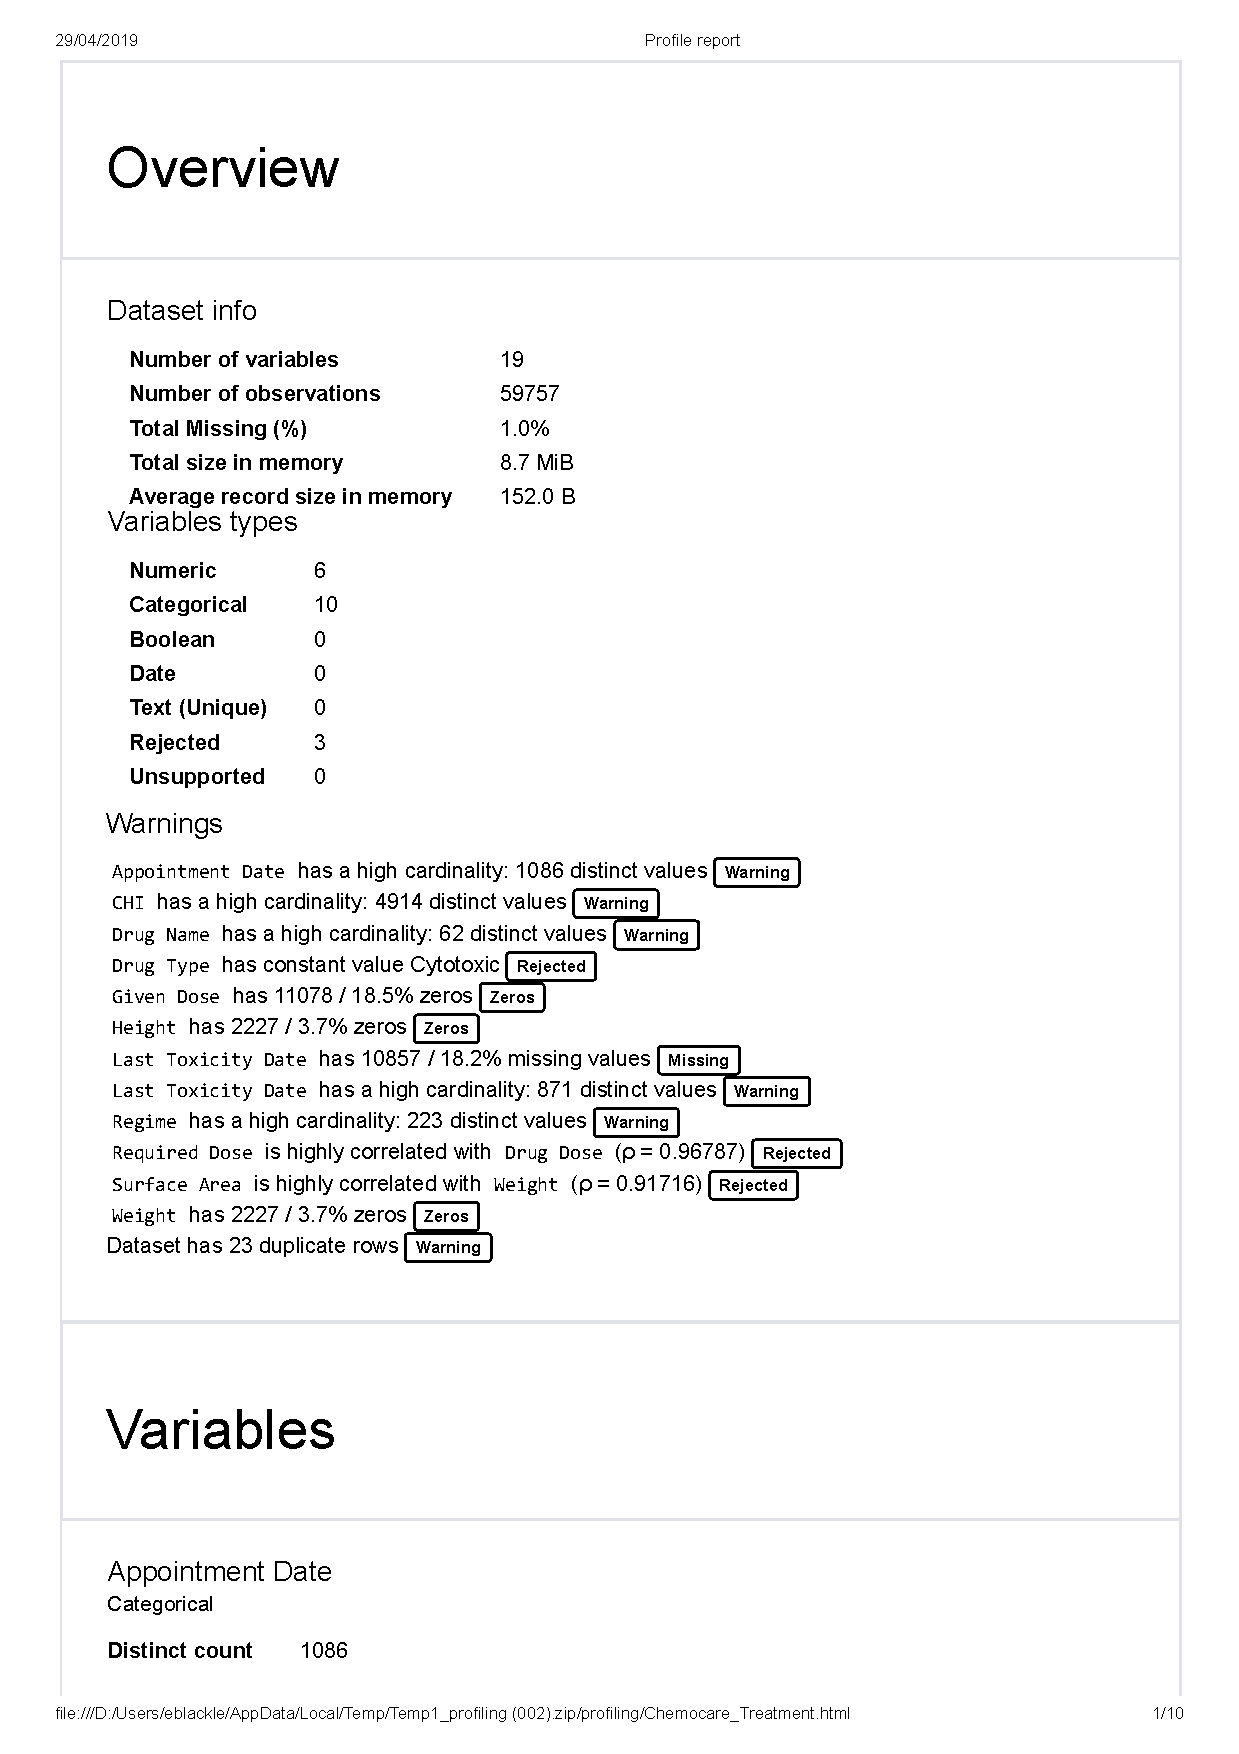
\includepdf[pages=-]{PDF/chemocare_treatment.pdf}
